 %!TEX program = latexmk
\documentclass[12pt,fleqn]{article}
\usepackage{setspace}
\usepackage{float}

\usepackage[english]{babel}
\PassOptionsToPackage{table,xcdraw}{xcolor}
\usepackage{xcolor}
\usepackage[utf8]{inputenc}
\usepackage[T1]{fontenc}


% A few common packages
\usepackage{amsmath}
\usepackage{amssymb}
\usepackage{amsthm}
\usepackage{array}
\usepackage{ifpdf}
\ifpdf
  \usepackage{graphicx}
\else
  \usepackage[dvipdfmx]{graphicx}
\fi
\usepackage{relsize}
\usepackage[titletoc]{appendix}
\usepackage{caption}
% \usepackage{xurl}
\captionsetup[table]{skip=10pt plus 0.01pt}
\usepackage{subcaption}  % \begin{subfigure}...\end{subfigure} within figure
\usepackage{multirow}
\usepackage{tabularx}
\usepackage{makecell}
\usepackage{booktabs}
% \usepackage{ltablex}
\usepackage[autostyle, english = american]{csquotes}


% Uncomment the following to attempt to enforce Type 1 or TrueType 
% fonts. ProQuest does not want the type 3 fonts used by default as
% of Dec. 2019 - see 
% https://support.proquest.com/articledetail?id=kA01W000000k9o2SAA . 
% If you are unable to embed fonts such as 'Zapf Dingbats' or 
% 'Symbol', try using raster images (.jpg or .png) instead of vector 
%images (.pdf or .eps).
% \usepackage[T1]{fontenc} 

% plainpages=false fixes the "duplicate ignored" error with page counters
% Set pdfborder to 0 0 0 to disable colored borders around PDF hyperlinks
\makeatletter
\renewcommand{\@biblabel}[1]{}
\renewcommand{\@cite}[2]{(#1\if@tempswa , #2\fi)}
\makeatother
\setlength{\emergencystretch}{3em}

\ifpdf
  \usepackage[plainpages=false,pdfborder={0 0 0}]{hyperref}
\else
  \usepackage[dvipdfmx,plainpages=false,pdfborder={0 0 0}]{hyperref}
\fi

\begin{document}

\begin{titlepage}
  \pagenumbering{alph}
  \centering
  \vspace*{2cm}
  {\LARGE\bfseries Modeling Decanalization with Homeostatic Reinforcement Learning\par}
  \vspace{2cm}
  {\large
    Joshua Clingo\textsuperscript{1,*} and Jeff Yoshimi\textsuperscript{1}\par
  }
  \vspace{0.5cm}
  {\small
    ORCID: Joshua Clingo \texttt{0009-0003-9377-1532}; Jeff Yoshimi \texttt{0000-0001-7327-5599}\par
  }
  \vspace{1cm}
  {\normalsize
    \textsuperscript{1}School of Social Sciences, Humanities and Arts, University of California, Merced\par
  }
  \vspace{1cm}
  {\normalsize
    \textsuperscript{*}Corresponding author: Joshua Clingo\\
    Email: jclingo@ucmerced.edu\par
  }
  \vfill
\end{titlepage}

\pagenumbering{arabic}

\begin{abstract}

  Living organisms continuously manage their homeostatic setpoints but sometimes fall into the ruts and grooves of an entrenched or canalized behavioral repertoire. Clinicians employ interventions, from psychoactive drugs to targeted stimulus regimes, to transiently decanalize entrenched behaviors and support more adaptive patterns. We present a computational model in which canalization is learned: a foraging agent builds a cognitive map and becomes increasingly confident about where food is. Policies trained with a homeostatic reinforcement learning (HRL) objective or a one-sided negative-feedback (NF) objective in a stable world were evaluated after the world changed: familiar resources degraded and better ones appeared elsewhere. Left undisturbed, 70\% of HRL agents became trapped, returning to failing resources, and precise beliefs made this worse. A temporary decanalization that relaxed the precision of the agent's beliefs and increased the randomness of its choices, without altering its physiology, released trapped agents and restored regulation, across four training seeds). Both relaxation and randomless contributed to the effect. Intermediate intensity worked best, and the HRL agent benefited far more than the NF agent. The model makes the canalization account of decanalizing interventions testable and provides predictions for when in what situations it could be beneficial.

\end{abstract}

\vspace{0.5em}
\noindent\textbf{Keywords:} canalization, decanalization, homeostatic reinforcement learning, foraging, psychedelics, altered states

\section{Introduction}

Organisms are constantly confronted with the trade-off between exploitation, the pursuit of known sources of reward, and exploration, the pursuit of uncertain sources of reward \cite{stephens_foraging_1986}. Although organisms ideally switch between exploration and exploitation at will and at optimal times \cite{pearson_decision_2014}, they often remain in one of those modes for too long or continue to cycle between them in non-optimal ways \cite{barack_neurocomputational_2016, addicott_primer_2017}. This can lead to habituated behavior patterns that are in conflict with their homeostatic needs \cite{bernard_lectures_1974}. From a dynamical systems perspective, organisms get stuck in the wells of fixed attractors, in the ruts and grooves of a ‘canalized’ landscape of behaviors \cite{waddington_canalization_1959, carhart-harris_canalization_2023}. The Bayesian perspective suggests that precise priors reduce the impact of new evidence, leading to repeated suboptimal behaviors and rigid response patterns \cite{carhart-harris_rebus_2019, carhart-harris_canalization_2023}. Work in reinforcement learning \cite{sutton_reinforcement_1998} has demonstrated that the interaction of meta-parameters and environmental factors can lead to reduced exploration and therefore over-exploitation of rewarding resources \cite{huys_mapping_2013}. These resources are discounted in perceived value, resulting in ‘observational overfitting’, where agents stop exploring altogether because they fixate on the wrong observational factors---resources that once were rewarding but are no longer rewarding \cite{song_observational_2019}.

The problem of hypercanalization (over-canalization) has been recognized in psychology, cognitive science \cite{lloyd_understanding_2023}, clinical practice \cite{addicott_primer_2017}, and integrative psychotherapy \cite{schiepek_self-organization_2014, schiepek_integrative_2015, schiepek_psychotherapy_2017}. In integrative psychotherapy, intentional shifts between decanalization and recanalization are central to the therapeutic process because they allow for the integration and reintegration of positive behavioral patterns. These theorists draw on dynamical systems theory, in particular Haken's synergetics \cite{haken_synergetics_1977}, as well as on control theory and cybernetics \cite{wiener_cybernetics_2019}, to model feedback-driven mental pathologies and possible interventions. Related frameworks include homeostatic setpoint management and allostasis \cite{sterling_allostasis_1988, sterling_allostasis_2012}. In homeostatic reinforcement learning \cite{keramati_homeostatic_2014}, complex behaviors emerge and stabilize over time through learning and the temporal discounting it affords. However, the learning process can backfire if the organism becomes observationally overfitted and relies on rigid expectations about possible rewards in its environment.

On canalization accounts, hypercanalized behaviors such as depression, anxiety, PTSD, substance use disorder, and OCD are said to result from overweighted priors \cite{carhart-harris_canalization_2023}, rigid and stubborn response patterns that canalize behavior toward a downward spiral of maladaptive, self-fulfilling, and self-destructive behavior \cite{scheffer_dynamical_2024}. This view has made its way into psychedelic-assisted psychotherapy, where psychedelics have been proposed to provide an entropic burst that destabilizes brain networks, leading to long-term psychological transformation \cite{carhart-harris_entropic_2014, hipolito_pattern_2023, girn_complex_2023}. These authors propose that focused destabilization during the psychotherapeutic process can address many otherwise intractable conditions marked by behavioral canalization.

Psychedelics may also precipitate critical period plasticity similar to plasticity in early development, leading to ``exquisite sensitivity to environmental input'' \cite[Abstract]{lepow_critical_2021}. This mirrors Juliani et al.'s (2024) description of acute shifts to inference, which, when supported by heightened metaplasticity, result in learning and relearning of the environment and actions that can manipulate it. This learning is made even stronger when the environment itself shifts during these critical periods.

For the most part, these ideas have remained metaphorical. Existing conceptualizations are often suggestive, but they rarely model their assumptions directly. Without a quantitative foundation, their explanatory value is limited. To address this gap, we developed a simulation that translates some of these assumptions into observable behavior. The aim is to render earlier conceptualizations into formal structures that can be quantified and compared, thereby sharpening the concepts, demonstrating their applicability to simulated agents, and exposing open questions that become visible only once the informal ideas are turned into a behavioral model.

Our working model of decanalization is inspired by work on the entropic brain \cite{carhart-harris_entropic_2014,carhart-harris_entropic_2018}, canalization, and Hipólito et al.'s (2023) pattern-breaking model. We also draw heavily on Juliani et al.'s “Deep CANALs” (2024), which directly extends the ``CANAL'' model \cite{carhart-harris_canalization_2023} and distinguishes overfitting in inference from loss of plasticity in learning, treating the intersection of overfitting and low plasticity as a source of psychopathology. According to Juliani et al., decanalization acutely alters synaptic weights, sensory observations, and metaplasticity: “[Acute decanalization] is a function of both the current environmental context (made partially available to the model through a sequence of sensory observations) and the state of the system within the synaptic weight landscape. The inferred set of beliefs in a given instance are a function of the location of the system within the neural activity landscape.” In our agent-based model, sensory observations are observations about internal and external states. Synaptic weights correspond to learned associations between states, actions, and rewards. Neural activity corresponds to short-term beliefs represented by the state variables of the solutions. Metaplasticity is represented by factors that alter the learning dynamics of the system.

Although hypercanalization is expressly maladaptive, it is more modestly rooted in behavioral persistence, which can reflect both learning within an organism and changes that its activities produce in the environment. Established routes can offer material advantages: marine snails following existing mucus trails reduce their own mucus production \cite{davies_energy_2007}, while leafcutter ants construct trails by removing obstacles encountered during travel \cite{bochynek_infrastructure_2019}. Such feedback is central to niche construction: organisms modify their environments, changing the conditions they subsequently encounter \cite{laland_niche_2016}. This reflects a broader point from embodied, embedded, enactive, and extended (4E) approaches to cognition: habits are not stored only in the head but are distributed across brain, body, and world \cite{barandiaran_genealogical_2014, newen_oxford_2018}. A worn path, a cleared trail, or a familiar routine is a behavioral pattern embodied in the environment, and it continues to shape behavior regardless of what the organism has learned. In real-world environments, agents learn against the backdrop of niche construction. We represent one aspect of this through introducing traversal costs that decrease with repeated visits. The advantage of niche construction is efficiency and reliability, but it can also lead to hypercanalization if the organism becomes over-reliant on a few sources of reward and fails to adapt to new surroundings.

In this paper, we model canalization as something an agent learns: confident beliefs about where resources are, formed while the world is stable. We test four hypotheses. First, canalization formed in a stable world becomes maladaptive when the world changes, trapping the agent in patterns that no longer serve its homeostatic needs. Second, a temporary decanalization that relaxes the precision of those beliefs and increases the variability of the agent's choices, without changing its physiology, releases it and improves subsequent regulation. Third, the intervention works best at an intermediate intensity---limited or excessive decanalization is unhelpful at best. Fourth, an agent trained with a homeostatic reinforcement learning (HRL) objective benefits more than one trained with a one-sided negative-feedback (NF) objective.

The contrast between HRL and NF follows Keramati and Gutkin (2014), who argued that homeostatic reinforcement learning, unlike classical negative-feedback accounts, explains anticipatory regulation. Intuitively, HRL resembles a heating and air-conditioning system that maintains a stable temperature; NF resembles a heater that acts only when the temperature falls below a fixed setpoint. An NF agent may escape an entrenched pattern as readily as an HRL agent, but only the HRL agent is rewarded for using its new freedom to stay near its setpoint.

\section{Methods}

We built a simulation in which an agent manages a single homeostatic variable while foraging in a two-dimensional world, learns where resources are, and becomes more confident in what it has learned. Canalization is represented by that confidence: the precision of the agent's beliefs about where food is. Decanalization is represented by a temporary relaxation of that precision, together with an increase in the randomness of the agent's choices, in line with the REBUS account of relaxed beliefs under psychedelics \cite{carhart-harris_rebus_2019} and the distinction between inference and behavioral variability in Deep CANALs \cite{juliani_deep_2024}.

An earlier version of this study used an Unreal Engine sandbox with a reactive policy and fixed perception. Analyses of that version showed that its agents did not form persistent, history-dependent routes: route overlap across phases was close to the level expected between unrelated trials, and manipulating the agent's tile history had little behavioral effect. Because there was no canal to disrupt, that version could not test decanalization (Supplementary Material, Sections~1--2). The present model was designed to supply the two missing ingredients: an agent whose behaviour depends on learned, history-dependent beliefs, and a world that changes after those beliefs form. The simulation is written in Python; its world mirrors the Unreal task where possible.

\subsection{World}\label{sec:world}

The world is a $50\times50$ toroidal grid of unit tiles. At each tick of $\Delta t=0.05$\,s the agent moves forward at 5 tiles\,s$^{-1}$ and turns by up to $10^\circ$. Its homeostatic state $h$ (setpoint 0) changes as
\begin{equation}\label{eq:h}
  h_{t+1}=h_t+o_t-\left(c(n_\tau)+\ell\right)\Delta t,
\end{equation}
where $o_t$ is the value of a pellet harvested during the tick, $\ell=2$ is a passive loss per second, and $c(n_\tau)$ is the traversal cost of the occupied tile, which falls with the tile's entry count $n_\tau$:
\begin{equation}\label{eq:wear}
  c(n)=c_{\min}+(c_0-c_{\min})\,e^{-n/k},\qquad c_0=5,\ c_{\min}=1,\ k=3.
\end{equation}
Entry counts fade with a half-life of 200\,s, so a worn path persists only through use.

Resources occur in ten patches of $3\times3$ cells, each with a quality drawn uniformly from $[3,15]$; each cell holds one pellet of that value. Harvested pellets regrow after a delay of $8\,\mathrm{s}/f$, where $f\in(0,1]$ is the patch's fertility. Every harvest multiplies $f$ by $0.92$, and $f$ recovers toward 1 with a time constant of 300\,s. Heavily used patches therefore regrow slowly: an exploited route stops paying.

We use two versions of the world. In the \emph{stable} world, patches never degrade and no new resources appear. In the \emph{changing} world, patches degrade as described, and at the start of the second phase two new, reliable patches appear at least 20 tiles from the agent's position at that moment. Reliable patches have ordinary quality (uniform $[8,12]$), never degrade, and regrow twice as fast. A canalized agent whose familiar patches are failing therefore has a better option available, outside the area it habitually uses.

\subsection{Agent: perception and cognitive map}\label{sec:map}

The agent perceives along seven rays spanning $90^\circ$ with a range of 10 tiles. Perception is fixed. The agent maintains a cognitive map with a believed pellet value $V_c$ and a precision $P_c$ for every cell $c$. Each observation of a cell, with value $v$ and observation precision $P_s$, updates the map by precision weighting:
\begin{equation}\label{eq:belief}
  V_c\leftarrow\frac{P_cV_c+P_sv}{P_c+P_s},\qquad P_c\leftarrow P_c+P_s .
\end{equation}
A cell in view contributes $P_s=0.05$ per tick, standing on a cell contributes $0.5$\,s$^{-1}$, and a harvest contributes $P_s=2$. Precision decays with a time constant of 200\,s. Cells that have repeatedly paid off therefore become precise, and later evidence that they are empty moves the belief only slowly: a precise prior about an exhausted patch continues to make it look rich. This is the model's locus of canalization. It is learned from experience, not imposed.

The agent also expects a harvested cell to regrow over 8\,s, so the believed worth of a cell is $V_c\,(1-e^{-(t-t_c)/8})$, where $t_c$ is the time of its last harvest. A patch that regrows more slowly than expected disappoints on each return; precise beliefs make the agent keep returning.

\subsection{Policy, objectives and training}\label{sec:policy}

Every 0.5\,s a learned policy chooses one of four options, each executed with fixed steering rules: \textsc{seek} the remembered cell with the greatest believed worth per unit distance; \textsc{explore} toward the nearest cell never seen; \textsc{cruise} along the cheapest (most worn) direction; or \textsc{avoid} visible food. The policy receives eleven inputs: $h$, the best remembered worth with its distance and precision, the value and distance of visible food, the distance to unexplored territory, map coverage, current traversal cost, time since the last harvest, and a bias term. It is a two-layer network of 64 units per layer with separate policy and value outputs.

Both objectives reward drive reduction \cite{keramati_homeostatic_2014}. With $D_t$ the drive at tick $t$, each tick earns $r_t=\kappa\,(D_{t-1}-D_t)$ with $\kappa=\Delta t/(1-\gamma)$ and $\gamma=0.99$, summed over the ticks of an option.
\begin{itemize}
  \item \textbf{Homeostatic reinforcement learning (HRL)}: $D=|h|/25$. Deviations in either direction are costly.
  \item \textbf{Negative feedback (NF)}: $D=\max(-h,0)/25$. Only deficits are costly; surplus earns nothing and is not penalized, like a heater that acts only below its setpoint.
\end{itemize}

\begin{sloppypar}
Policies were trained with proximal policy optimization \cite{schulman_proximal_2017} for 60 iterations of 16 trials (about 1.3 million decisions), in the stable world, without any intervention. For each objective, four independent training seeds were run. A checkpoint was selected for each seed from every fifth iteration (from iteration 20) and the last, on eight held-out stable-world trials, by the family's own objective: lowest mean $|h|$ for HRL and lowest mean deficit for NF. Settings are listed in Appendix~\ref{app:implementation-settings}. Weights are fixed during evaluation.
\end{sloppypar}

\subsection{Canalization, decanalization and recanalization}\label{sec:protocol}

Each evaluation trial has three phases: 300\,s of canalization, 100\,s of intervention, and 300\,s of recanalization. The trial runs in the changing world, so the policy, trained in a stable world, meets degradation and new resources it was never trained on. The homeostatic state is continuous across phases: because the intervention does not alter physiology, carrying $h$ over does not confound the comparison.

In the CCC condition, the agent is left undisturbed. In the CDR condition, decanalization with dose $d\in[0,1]$ is applied during the second phase through two levers:
\begin{itemize}
  \item \textbf{Relaxed precision}: at the start of the window, every belief's precision is multiplied by $1-d$. During the window, new evidence is weighed against priors of precision $(1-d)P_c$. The agent's beliefs become easier to revise.
  \item \textbf{Increased behavioral entropy}: the policy's sampling temperature is raised to $1+b\,d$, where $b$ is the entropy \emph{boost}. The agent's option choices become more variable.
\end{itemize}
We evaluated $b\in\{0,1,3\}$ and $d\in\{0.5,1\}$, and $b=10$ at $d=1$; and, to separate the levers, entropy alone ($b\in\{1,3\}$ with precision unchanged). As a reference for the cost of canalization, we also evaluated each policy with beliefs that track the senses (no harvest precision, precision time constant 20\,s; ``low precision'').

\subsection{Endpoints and statistics}\label{sec:stats}

The primary endpoint is the phase-3 mean absolute deviation of $h$ from the setpoint (MAE). A phase counts as \emph{trapped} if $h$ falls to $-100$ or below. We also report harvests from the newly appeared patches. Each training seed was evaluated on 64 paired trials (evaluation seeds 5000--5063): paired trials share the world layout, starting state and random streams, so condition differences within a seed are paired. Because conclusions should generalize across training runs, the training seed is the unit of inference: per-seed mean differences are averaged across the four seeds, with 95\% $t$-intervals ($df=3$). Criteria for each test were fixed before the corresponding run. Model development preceded these runs and used separate seeds; that history, including decisions made after seeing data, is reported in the Supplementary Material.

\subsection{Code and data availability}

The simulation, training and analysis code and the evaluation outputs are available at \url{https://github.com/JClingo/decanalization}.

\section{Results}\label{model-results}

\subsection{Canalization becomes hypercanalization when the world changes}

Trained in a stable world, both policies regulate agents well. In the changing world, left undisturbed, they become trapped: as familiar patches degrade, the agents keep pursuing them, and $h$ falls. Across training seeds, 70\% of HRL trials (95\% CI [66, 73]) and 48\% of NF trials ([44, 51]) were trapped in phase 3 (Table~\ref{tab:main}). Precise beliefs made this worse. The same policies with beliefs that track the senses regulated better: HRL phase-3 MAE was 60 points higher with learned precision ([43, 78]), and NF trapping was 0.33 higher ([0.25, 0.41]).

Trapping depends on the world having changed in ways the policy did not anticipate. An HRL policy trained in the changing world itself was almost never trapped (2\%) and regulated near the noise floor (phase-3 MAE 12.5); decanalization then had nothing to improve (difference $-0.7$, 95\% CI $[-1.9, 0.8]$; one training seed).

\begin{figure}[htbp]
\centering
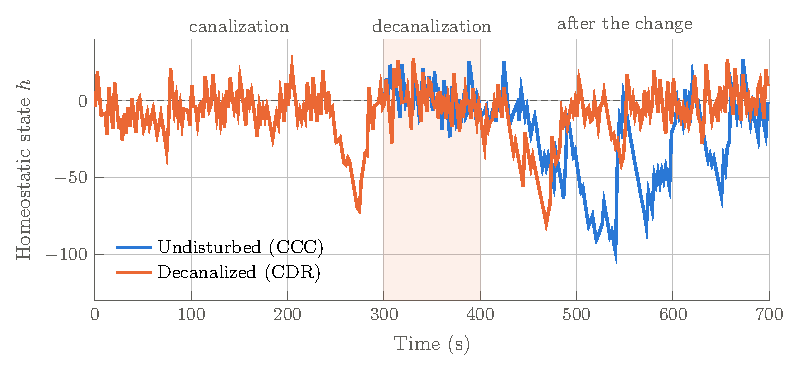
\includegraphics[width=\linewidth]{figures/trajectory.pdf}
\caption{One paired trial (HRL, stable-trained). Both agents follow the same trajectory until the intervention. Left undisturbed, the agent keeps returning to its depleted patches after the world changes, and its state falls to about $-100$; decanalized for 100\,s, it dips once, finds the new resources, and returns to the setpoint.}
\label{fig:trajectory}
\end{figure}

\subsection{Decanalization releases trapped agents}

Decanalization during the second phase restored regulation in the HRL agent (Table~\ref{tab:main}, Figure~\ref{fig:trajectory}). With relaxed precision and an entropy boost of 1, phase-3 MAE fell by 83 points ([77, 89]); every training seed showed a reduction between 78 and 86. With an entropy boost of 3 it fell by 98 ([73, 122]). Trapping fell by 23 percentage points, and the improvement reached typical trials, not only the trapped tail: in the first training seed, median phase-3 MAE fell from 81 to 14. Smaller doses had smaller effects ($d=0.5$: $-43$ and $-63$ at boosts 1 and 3).

\begin{table}[htbp]
\centering\small
\renewcommand{\arraystretch}{1.15}
\begin{tabularx}{\linewidth}{@{}>{\raggedright\arraybackslash}Xrr@{}}
\toprule
 & HRL & NF\\
\midrule
Trapped in phase 3, undisturbed & 0.70 [0.66, 0.73] & 0.48 [0.44, 0.51]\\
Phase-3 MAE, undisturbed & 136 [119, 153] & 172 [96, 247]\\
Precision cost: MAE, learned minus low precision & $+60$ [43, 78] & $+27$ [$-12$, 66]\\
Decanalization, boost 1, $d=1$: $\Delta$MAE & $-83$ [$-89$, $-77$] & $-34$ [$-54$, $-14$]\\
\quad $\Delta$ trapped & $-0.23$ [$-0.34$, $-0.12$] & $-0.33$ [$-0.39$, $-0.28$]\\
Decanalization, boost 3, $d=1$: $\Delta$MAE & $-98$ [$-122$, $-73$] & $-28$ [$-58$, 2]\\
Decanalization, boost 10, $d=1$: $\Delta$MAE$^{a}$ & $-72$ [$-100$, $-44$] & $-9$ [$-14$, $-4$]\\
Phase-2 MAE at boosts 1 / 3 / 10 & 66 / 62 / 108 & 91 / 108 / 139\\
\bottomrule
\end{tabularx}
\caption{Main results in the changing world for policies trained in the stable world. Means across four training seeds with 95\% $t$-intervals over seeds; each seed contributes 64 paired trials. $\Delta$ is decanalized minus undisturbed. $^{a}$Three training seeds.}
\label{tab:main}
\end{table}

\subsection{Both levers contribute}

Either lever alone released a substantial share of trapped HRL agents (Figure~\ref{fig:levers}). Relaxing belief precision without changing behavioral entropy reduced phase-3 MAE by 59 points ([41, 76]); raising entropy alone reduced it by 11 ([3, 19]) at a boost of 1 and by 61 ([49, 73]) at a boost of 3. Combined, the levers were most effective. At a boost of 1 the combination exceeded the sum of its parts ($-83$ against $-70$); at a boost of 3 it fell short of the sum ($-98$ against $-120$), indicating that the two levers partly act through the same route: they let the agent leave patches its beliefs still favor.

\begin{figure}[htbp]
\centering
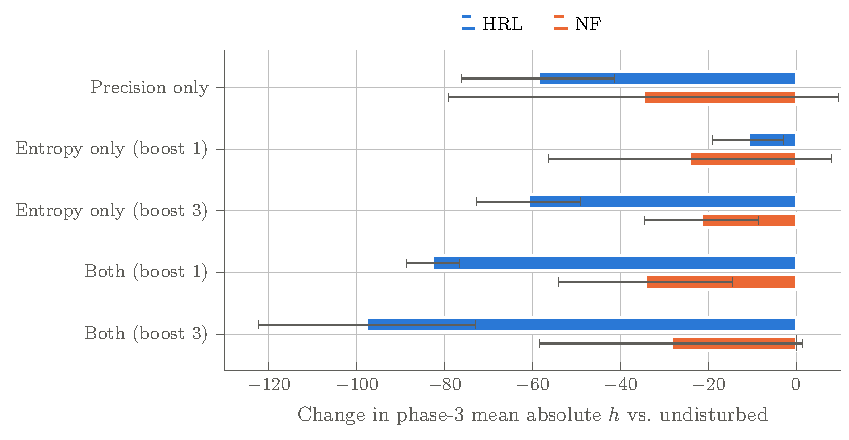
\includegraphics[width=\linewidth]{figures/levers.pdf}
\caption{Effect of each decanalization lever on phase-3 mean absolute $h$ (decanalized minus undisturbed; $d=1$ for 100\,s). Bars show means across four training seeds; error bars show 95\% $t$-intervals over seeds. Negative values are improvements.}
\label{fig:levers}
\end{figure}

\subsection{An intermediate intensity works best}

Extreme behavioral perturbation was not ideal. With precision relaxed, raising the entropy boost from 3 to 10 reduced the benefit by 18 points ([5, 31]), and the cost during the intervention rose sharply: phase-2 MAE was 108 at a boost of 10 against 62 at a boost of 3. The most disruptive setting tested was still better than no intervention, so the model shows diminishing and then declining returns rather than outright harm.

\subsection{HRL benefits more than NF}

Decanalization reduced trapping in the NF agent as well (by 33 percentage points at a boost of 1), and NF agents also found the new resources. Their regulation improved much less: phase-3 MAE fell by 34 points ([14, 54]) at a boost of 1, and the effect shrank toward zero at higher boosts. Paired by trial, the HRL improvement exceeded the NF improvement by 48 points ([29, 68]); every training seed showed the difference. NF rewards only the removal of deficits, so an NF agent that escapes a failing patch has no incentive to avoid overshooting once fed; its absolute deviation is dominated by surplus.

\section{Discussion}\label{model-discussion}

We hypothesized that decanalization would improve post-intervention homeostatic regulation in an HRL agent, and that an NF agent would benefit less. Both predictions held, in a model where canalization demonstrably exists. Canalization here is a learned property: an agent that gathers food reliably in a stable world becomes confident about where food is. That confidence is efficient while the world stays the same. When the world changes, the same confidence holds the agent to patches that no longer pay, even as better resources appear elsewhere: hypercanalization, in the sense of maladaptive persistence after the conditions that justified a habit have gone \cite{carhart-harris_canalization_2023}. Agents with less precise beliefs, or policies that had been trained on the change, were rarely trapped.

\begin{sloppypar}
Decanalization acted on here canalization is stored. Relaxing the precision of beliefs---the core of the REBUS account \cite{carhart-harris_rebus_2019}---let new evidence revise the agent's map; increasing the entropy of its choices let it sample options its beliefs disfavored. Each lever helped on its own, and their combination helped most, consistent with the distinction in Deep CANALs between rigid inference and reduced behavioral variability \cite{juliani_deep_2024}. Neither lever changed the agent's physiology, the reward function, or its learned weights; the benefit came from what the agent did with a temporarily loosened view of its world, and persisted after the intervention ended.
\end{sloppypar}

Intermediate decanalization was the most effective. Strong behavioral perturbation disorganized foraging during the window and left the agent worse off afterwards than a moderate perturbation did. This is the shape predicted by analogies with simulated annealing \cite{kirkpatrick_optimization_1983, hajek_cooling_1988}: destabilization helps when it is enough to leave a poor attractor but not so much that useful structure is lost. In a heuristic version of the agent, without a learned policy, sufficiently strong exploration made outcomes worse than no intervention at all; with learned policies, the strongest setting we tested was still beneficial.

The HRL--NF difference follows from the objectives. Both agents escaped their failing patches, but only the HRL agent is rewarded for staying near its setpoint once it does. Decanalization creates an opportunity; whether the opportunity improves regulation depends on what the agent is trying to regulate. This is the contrast motivated by Keramati and Gutkin's comparison of homeostatic and negative-feedback accounts \cite{keramati_homeostatic_2014}.

\subsection{Limitations}

The decanalization levers, the option set, and the cognitive map are modeling choices. They are motivated by the REBUS and CANAL frameworks, but other formalizations of ``relaxed priors'' are possible, and the results show what follows from these ones. The model does not learn during or after the intervention: its weights are fixed, and the lasting effect of decanalization runs entirely through the agent's beliefs and position in the world.

Hypercanalization required that the world change in ways the policy had not been trained on. This is part of the theory rather than a convenience, but it means the effect size depends on the size of that mismatch, which we did not explore. The changing world also supplies a better alternative; without one, escaping a failing patch is less useful, and in development runs without new resources, decanalization rarely improved regulation (Supplementary Material, Section~4).

Four training seeds per objective support generalization across training runs, but not across architectures or hyperparameters. NF regulation is dominated by surplus, which its objective does not penalize; NF results are best read through trapping. The drive-reduction rewards omit the finite-endpoint correction used in our earlier Unreal implementation, and checkpoints were selected on held-out trials of the training world. Finally, the model manages a single setpoint in a simple world. It should be read as a formal demonstration of one mechanism, not as an account of psychiatric conditions or of psychedelic treatment.
% TODO: Fix up this NF section since it's a bit off


\subsection{Future Directions}

The present study applies one intervention to agents whose weights are fixed. Allowing learning during and after the intervention would test whether a decanalized agent consolidates the new route into its policy, as accounts of critical-period plasticity suggest \cite{nardou_psychedelics_2023}. Repeated cycles of change and intervention would show whether there is an optimal schedule, and whether repeated decanalization eventually prevents useful canalization. The conditions after the intervention also matter \cite{carhart-harris_context_2018}: varying whether better alternatives exist, and how far away they are, would map when decanalization helps and when it only costs.

\section{Conclusions}

Research on canalization and decanalization often moves between clinical, dynamical and mechanistic vocabularies without making the underlying computational assumptions explicit. We formalized one set of them. An agent that learns confident beliefs about its world in stable conditions becomes trapped when the world changes; temporarily relaxing the precision of those beliefs and the regularity of its choices releases it, restores its homeostatic regulation, and works best at an intermediate intensity. The benefit is much larger for an agent that values staying near its setpoint than for one that only avoids deficits. These results make the canalization account testable in a simulated agent, and they identify the conditions under which decanalization should help: when entrenched beliefs keep an agent from options that would now serve it better.

Like most scientific models, ours is a simplified approximation of a much more complex reality, and many technical and parameter choices shaped the results. The model should therefore be read as a formal demonstration of one candidate mechanism, not as a direct account of psychiatric disorders, psychotherapeutic change, or psychedelic treatment outcomes.

\section*{Declarations}

\subsection*{Declaration of conflicting interests}
The authors declare that there is no conflict of interest.

\subsection*{Funding}
\begin{sloppypar}
  The authors received no financial support for the research, authorship, and/or publication of this article.
\end{sloppypar}

\subsection*{Use of AI}

The authors used AI agents to assist with analysis code, implementation audits, and manuscript revision. During revision, AI assisted with checking the source repository and evaluation records, regenerating tables, integrating revised methods and results, and providing suggestions for manuscript text. All content was thoroughly reviewed, edited, and approved by the authors.

\subsection*{Ethics approval}
Not applicable. This study used only simulated agents in a simulated environment; no human participants, nonhuman animals, biological specimens, or clinical records were involved.

\subsection*{Data and code availability}
The simulation, training and analysis code and the evaluation outputs used in this study are openly available at \url{https://github.com/JClingo/decanalization}. The earlier Unreal Engine sandbox is archived in the same repository (\texttt{archive/unreal}; tag \texttt{unreal-v1}).

\sloppy
\begin{thebibliography}{33}
  \providecommand{\natexlab}[1]{#1}
  \providecommand{\url}[1]{\texttt{#1}}
  \expandafter\ifx\csname urlstyle\endcsname\relax
    \providecommand{\doi}[1]{doi: #1}\else
    \providecommand{\doi}{doi: \begingroup \urlstyle{rm}\Url}\fi

  \bibitem[Addicott et~al., 2017]{addicott_primer_2017}
  M.~A. Addicott, J.~M. Pearson, M.~M. Sweitzer, D.~L. Barack, and M.~L. Platt.
  \newblock A primer on foraging and the explore/exploit trade-off for psychiatry
  research.
  \newblock 42\penalty0 (10):\penalty0 1931--1939, 2017.
  \newblock ISSN 1740-634X.
  \newblock \doi{10.1038/npp.2017.108}.
  \newblock URL \url{https://www.nature.com/articles/npp2017108}.
  \newblock Publisher: Nature Publishing Group.

  \bibitem[Badia et~al., 2020]{badia_agent57_2020}
  Adri\`a~Puigdom\`enech Badia, Bilal Piot, Steven Kapturowski, Pablo
  Sprechmann, Alex Vitvitskyi, Daniel Guo, and Charles Blundell.
  \newblock Agent57: Outperforming the {Atari} human benchmark.
  \newblock In \emph{Proceedings of the 37th International Conference on
  Machine Learning}, volume 119 of \emph{Proceedings of Machine Learning
  Research}, pages 507--517, 2020.

  \bibitem[Barandiaran and Di~Paolo, 2014]{barandiaran_genealogical_2014}
  Xabier~E. Barandiaran and Ezequiel~A. Di~Paolo.
  \newblock A genealogical map of the concept of habit.
  \newblock 8:\penalty0 522, 2014.
  \newblock \doi{10.3389/fnhum.2014.00522}.
  \newblock URL
  \url{https://www.frontiersin.org/articles/10.3389/fnhum.2014.00522}.

  \bibitem[Barack and Platt, 2016]{barack_neurocomputational_2016}
  David~L. Barack and Michael~L. Platt.
  \newblock Neurocomputational nosology: {{Malfunctions}} of models and
  mechanisms.
  \newblock \emph{Frontiers in Psychology}, Volume 7 - 2016, 2016.
  \newblock ISSN 1664-1078.
  \newblock \doi{10.3389/fpsyg.2016.00602}.

  \bibitem[Barak, 2017]{barak_recurrent_2017}
  Omri Barak.
  \newblock Recurrent neural networks as versatile tools of neuroscience
  research.
  \newblock 46:\penalty0 1--6, 2017.
  \newblock ISSN 0959-4388.
  \newblock \doi{10.1016/j.conb.2017.06.003}.
  \newblock URL
  \url{https://www.sciencedirect.com/science/article/pii/S0959438817300429}.

  \bibitem[Bathje et~al., 2022]{bathje_psychedelic_2022}
  Geoff~J. Bathje, Eric Majeski, and Mesphina Kudowor.
  \newblock Psychedelic integration: An analysis of the concept and its practice.
  \newblock 13, 2022.
  \newblock ISSN 1664-1078.
  \newblock URL
  \url{https://www.frontiersin.org/articles/10.3389/fpsyg.2022.824077}.

  \bibitem[Bernard, 1974]{bernard_lectures_1974}
  C.~Bernard.
  \newblock \emph{Lectures on the phenomena of life common to animals and
    plants}.
  \newblock American lecture series, publication. Thomas, 1974.
  \newblock ISBN 978-0-398-02857-2.
  \newblock URL \url{https://books.google.com/books?id=zMhqAAAAMAAJ}.
  \newblock Number: v. 1 tex.lccn: 73004297.

  \bibitem[Bochynek et~al., 2019]{bochynek_infrastructure_2019}
  Thomas Bochynek, Martin Burd, Christoph Kleineidam, and Bernd Meyer.
  \newblock Infrastructure construction without information exchange: the trail
  clearing mechanism in \emph{Atta} leafcutter ants.
  \newblock \emph{Proceedings of the Royal Society B: Biological Sciences},
  286(1895):20182539, 2019.
  \newblock \doi{10.1098/rspb.2018.2539}.

  \bibitem[Brouwer and Carhart-Harris, 2021]{brouwer_pivotal_2021}
  Ari Brouwer and Robin~L. Carhart-Harris.
  \newblock Pivotal mental states.
  \newblock \emph{Journal of Psychopharmacology}, 35(4):319--352, 2021.
  \newblock \doi{10.1177/0269881120959637}.

% SUGGESTED EDIT [24]: Proposed supporting reference: brouwer_trajectory_2024.
%   \bibitem[Brouwer et~al., 2024]{brouwer_trajectory_2024}
%   Ari Brouwer, Joshua K. Brown, Earth Erowid, Fire Erowid, Sylvia Thyssen,
%   Charles L. Raison, and Robin L. Carhart-Harris.
%   \newblock The temporal trajectory of the psychedelic mushroom experience
%   mimics the narrative arc of the Hero's Journey.
%   \newblock \emph{Research Square}, preprint, version 1, 2024.
%   \newblock \doi{10.21203/rs.3.rs-3941205/v1}.
% END SUGGESTED EDIT [24]
  \bibitem[Carhart-Harris and Friston, 2019]{carhart-harris_rebus_2019}
  R.~L. Carhart-Harris and K.~J. Friston.
  \newblock {REBUS} and the anarchic brain: Toward a unified model of the brain
  action of psychedelics.
  \newblock 71\penalty0 (3):\penalty0 316--344, 2019.
  \newblock ISSN 0031-6997.
  \newblock \doi{10.1124/pr.118.017160}.
  \newblock URL \url{https://www.ncbi.nlm.nih.gov/pmc/articles/PMC6588209/}.

  \bibitem[Carhart-Harris et~al., 2023]{carhart-harris_canalization_2023}
  R.~L. Carhart-Harris, S.~Chandaria, D.~E. Erritzoe, A.~Gazzaley, M.~Girn,
  H.~Kettner, P.~A.~M. Mediano, D.~J. Nutt, F.~E. Rosas, L.~Roseman,
  C.~Timmermann, B.~Weiss, R.~J. Zeifman, and K.~J. Friston.
  \newblock Canalization and plasticity in psychopathology.
  \newblock 226:\penalty0 109398, 2023.
  \newblock ISSN 0028-3908.
  \newblock \doi{10.1016/j.neuropharm.2022.109398}.
  \newblock URL
  \url{https://www.sciencedirect.com/science/article/pii/S0028390822004579}.

  \bibitem[Carhart-Harris et~al., 2014]{carhart-harris_entropic_2014}
  Robin Carhart-Harris, Robert Leech, Peter Hellyer, Murray Shanahan, Amanda
  Feilding, Enzo Tagliazucchi, Dante Chialvo, and David Nutt.
  \newblock The entropic brain: a theory of conscious states informed by
  neuroimaging research with psychedelic drugs.
  \newblock 8, 2014.
  \newblock ISSN 1662-5161.
  \newblock URL
  \url{https://www.frontiersin.org/article/10.3389/fnhum.2014.00020}.

  \bibitem[Carhart-Harris, 2018]{carhart-harris_entropic_2018}
  Robin~L. Carhart-Harris.
  \newblock The entropic brain---revisited.
  \newblock 142:\penalty0 167--178, 2018.
  \newblock ISSN 0028-3908.
  \newblock \doi{10.1016/j.neuropharm.2018.03.010}.
  \newblock URL
  \url{https://www.sciencedirect.com/science/article/pii/S0028390818301175}.

  \bibitem[Carhart-Harris et~al., 2018]{carhart-harris_context_2018}
  Robin~L. Carhart-Harris, Leor Roseman, Eline Haijen, David Erritzoe,
  Rosalind Watts, Igor Branchi, and Mendel Kaelen.
  \newblock Psychedelics and the essential importance of context.
  \newblock \emph{Journal of Psychopharmacology}, 32(7):725--731, 2018.
  \newblock \doi{10.1177/0269881118754710}.

  \bibitem[Clingo, 2025]{clingoDisintegrationReintegrationModelPsychological2025}
  Joshua Clingo.
  \newblock \emph{The Disintegration-Reintegration Model of Psychological Transformation}.
  \newblock Thesis, UC Merced, July 23, 2025.
  \newblock URL \url{https://escholarship.org/uc/item/54z4d95j}.

  \bibitem[Davies and Blackwell, 2007]{davies_energy_2007}
  Mark~S. Davies and Janine Blackwell.
  \newblock Energy saving through trail following in a marine snail.
  \newblock \emph{Proceedings of the Royal Society B: Biological Sciences},
  274(1614):1233--1236, 2007.
  \newblock \doi{10.1098/rspb.2007.0046}.

  \bibitem[Girn et~al., 2023]{girn_complex_2023}
  Manesh Girn, Fernando~E. Rosas, Richard~E. Daws, Courtney~L. Gallen, Adam
  Gazzaley, and Robin~L. Carhart-Harris.
  \newblock A complex systems perspective on psychedelic brain action.
  \newblock 27\penalty0 (5):\penalty0 433--445, 2023.
  \newblock ISSN 1364-6613, 1879-307X.
  \newblock \doi{10.1016/j.tics.2023.01.003}.
  \newblock URL
  \url{https://www.cell.com/trends/cognitive-sciences/abstract/S1364-6613(23)00021-9}.
  \newblock Publisher: Elsevier.

  \bibitem[Haken, 1977]{haken_synergetics_1977}
  Hermann Haken.
  \newblock \emph{Synergetics: An Introduction. Nonequilibrium Phase Transitions
  and Self-Organization in Physics, Chemistry and Biology}.
  \newblock Springer, Berlin, 1977.

  \bibitem[Hajek, 1988]{hajek_cooling_1988}
  Bruce Hajek.
  \newblock Cooling schedules for optimal annealing.
  \newblock \emph{Mathematics of Operations Research}, 13(2):311--329, 1988.
  \newblock \doi{10.1287/moor.13.2.311}.

  \bibitem[Hayes et~al., 2007]{hayes_change_2007}
  Adele~M. Hayes, Jean-Philippe Laurenceau, Greg Feldman, Jennifer~L. Strauss,
  and LeeAnn Cardaciotto.
  \newblock Change is not always linear: The study of nonlinear and
  discontinuous patterns of change in psychotherapy.
  \newblock \emph{Clinical Psychology Review}, 27(6):715--723, 2007.
  \newblock \doi{10.1016/j.cpr.2007.01.008}.

  \bibitem[Hip\'olito et~al., 2023]{hipolito_pattern_2023}
  In\^es Hip\'olito, Jonas Mago, Fernando~E Rosas, and Robin Carhart-Harris.
  \newblock Pattern breaking: a complex systems approach to psychedelic medicine.
  \newblock 2023\penalty0 (1):\penalty0 niad017, 2023.
  \newblock ISSN 2057-2107.
  \newblock \doi{10.1093/nc/niad017}.
  \newblock URL \url{https://doi.org/10.1093/nc/niad017}.

  \bibitem[Hoffmann et~al., 2022]{hoffmann_training_2022}
  Jordan Hoffmann, Sebastian Borgeaud, Arthur Mensch, Elena Buchatskaya, Trevor
  Cai, Eliza Rutherford, Diego de~Las~Casas, Lisa~Anne Hendricks, Johannes
  Welbl, Aidan Clark, et~al.
  \newblock Training compute-optimal large language models.
  \newblock In \emph{Advances in Neural Information Processing Systems},
  volume~35, pages 30016--30030, 2022.

  \bibitem[Huys et~al., 2013]{huys_mapping_2013}
  Quentin~JM Huys, Diego~A. Pizzagalli, Ryan Bogdan, and Peter Dayan.
  \newblock Mapping anhedonia onto reinforcement learning: A behavioral
  meta-analysis.
  \newblock \emph{Biology of Mood \& Anxiety Disorders}, 3\penalty0 (1):\penalty0
  12, June 2013.
  \newblock ISSN 2045-5380.
  \newblock \doi{10.1186/2045-5380-3-12}.

  \bibitem[Juliani et~al., 2024]{juliani_deep_2024}
  Arthur Juliani, Adam Safron, and Ryota Kanai.
  \newblock Deep {CANALs}: a deep learning approach to refining the canalization
  theory of psychopathology.
  \newblock 2024\penalty0 (1):\penalty0 niae005, 2024.
  \newblock ISSN 2057-2107.
  \newblock \doi{10.1093/nc/niae005}.
  \newblock URL \url{https://doi.org/10.1093/nc/niae005}.

  \bibitem[Keramati and Gutkin, 2014]{keramati_homeostatic_2014}
  Mehdi Keramati and Boris Gutkin.
  \newblock Homeostatic reinforcement learning for integrating reward collection
  and physiological stability.
  \newblock 3:\penalty0 e04811, 2014.
  \newblock ISSN 2050-084X.
  \newblock \doi{10.7554/eLife.04811}.
  \newblock URL \url{https://doi.org/10.7554/eLife.04811}.
  \newblock Publisher: {eLife} Sciences Publications, Ltd.

  \bibitem[Kirkpatrick et~al., 1983]{kirkpatrick_optimization_1983}
  S. Kirkpatrick, C.~D. Gelatt, Jr., and M.~P. Vecchi.
  \newblock Optimization by simulated annealing.
  \newblock \emph{Science}, 220(4598):671--680, 1983.
  \newblock \doi{10.1126/science.220.4598.671}.

  \bibitem[Laland et~al., 2016]{laland_niche_2016}
  Kevin Laland, Blake Matthews, and Marcus W. Feldman.
  \newblock An introduction to niche construction theory.
  \newblock \emph{Evolutionary Ecology}, 30:191--202, 2016.
  \newblock \doi{10.1007/s10682-016-9821-z}.

  \bibitem[Lepow et~al., 2021]{lepow_critical_2021}
  Lauren Lepow, Hirofumi Morishita, and Rachel Yehuda.
  \newblock Critical period plasticity as a framework for psychedelic-assisted
  psychotherapy.
  \newblock 15, 2021.
  \newblock ISSN 1662-453X.
  \newblock \doi{10.3389/fnins.2021.710004}.
  \newblock URL
  \url{https://www.frontiersin.org/journals/neuroscience/articles/10.3389/fnins.2021.710004/full}.
  \newblock Publisher: Frontiers.

  \bibitem[Lloyd et~al., 2023]{lloyd_understanding_2023}
  Alex Lloyd, Essi Viding, Ryan McKay, and Nicholas Furl.
  \newblock Understanding patch foraging strategies across development.
  \newblock 27\penalty0 (11):\penalty0 1085--1098, 2023.
  \newblock ISSN 1364-6613, 1879-307X.
  \newblock \doi{10.1016/j.tics.2023.07.004}.
  \newblock URL
  \url{https://www.cell.com/trends/cognitive-sciences/abstract/S1364-6613(23)00172-9}.

  \bibitem[Lyon et~al., 2021]{lyon_reframing_2021}
  Pamela Lyon, Fred Keijzer, Detlev Arendt, and Michael Levin.
  \newblock Reframing cognition: getting down to biological basics.
  \newblock 376\penalty0 (1820):\penalty0 20190750, 2021.
  \newblock \doi{10.1098/rstb.2019.0750}.
  \newblock URL
  \url{https://royalsocietypublishing.org/doi/10.1098/rstb.2019.0750}.
  \newblock Publisher: Royal Society.

  \bibitem[Mnih et~al., 2015]{mnih_human-level_2015}
  Volodymyr Mnih, Koray Kavukcuoglu, David Silver, Andrei~A. Rusu, Joel Veness,
  Marc~G. Bellemare, Alex Graves, Martin Riedmiller, Andreas~K. Fidjeland,
  Georg Ostrovski, et~al.
  \newblock Human-level control through deep reinforcement learning.
  \newblock \emph{Nature}, 518(7540):529--533, 2015.
  \newblock \doi{10.1038/nature14236}.

  \bibitem[Moreno et~al., 2026]{moreno_randomized_2026}
  Francisco~A. Moreno, Katja~E. Allen, Christopher~B. Wiegand, Rajan Dunne,
  James~I. Prickett, Brian Bayze, and John~J.~B. Allen.
  \newblock A randomized clinical trial of repeated doses of psilocybin for
  the treatment of obsessive--compulsive disorder.
  \newblock \emph{Journal of Psychopharmacology}, 40(5):837--849, 2026.
  \newblock \doi{10.1177/02698811261424214}.

  \bibitem[Nardou et~al., 2023]{nardou_psychedelics_2023}
  Romain Nardou, Edward Sawyer, Young~Jun Song, Makenzie Wilkinson,
  Yasmin Padovan-Hernandez, J\'unia~Lara de~Deus, Noelle Wright, Carine Lama,
  Sehr Faltin, Loyal~A. Goff, Genevieve~L. Stein-O'Brien, and G\"ul D\"olen.
  \newblock Psychedelics reopen the social reward learning critical period.
  \newblock \emph{Nature}, 618(7966):790--798, 2023.
  \newblock \doi{10.1038/s41586-023-06204-3}.

  \bibitem[Newen et~al., 2018]{newen_oxford_2018}
  Albert Newen, Leon De~Bruin, and Shaun Gallagher, editors.
  \newblock \emph{The Oxford Handbook of 4E Cognition}.
  \newblock Oxford University Press, 2018.
  \newblock \doi{10.1093/oxfordhb/9780198735410.001.0001}.

  \bibitem[Paul, 2014]{paul_transformative_2014}
  L.~A. Paul.
  \newblock \emph{Transformative Experience}.
  \newblock Oxford University Press, Oxford, 2014.

  \bibitem[Pearson et~al., 2014]{pearson_decision_2014}
  John~M Pearson, Karli~K Watson, and Michael~L Platt.
  \newblock Decision making: the neuroethological turn.
  \newblock \emph{Neuron}, 82\penalty0 (5):\penalty0 950--965, June 2014.

  \bibitem[Pio-Lopez et~al., 2025]{pio-lopez_scale-free_2025}
  L\'eo Pio-Lopez, Giovanni Pezzulo, and Michael Levin.
  \newblock Scale-free niche construction: expanding agent-microenvironment
  co-development to unconventional substrates, 2025.
  \newblock URL \url{https://osf.io/ytg35_v1}.

  \bibitem[Safron and DeYoung, 2021]{safron_deyoung_2021}
  Adam Safron and Colin G. DeYoung.
  \newblock Integrating Cybernetic Big Five Theory with the free energy
  principle: A new strategy for modeling personalities as complex systems.
  \newblock In D. Wood, S. J. Read, P. D. Harms, and A. Slaughter, editors,
  \emph{Measuring and Modeling Persons and Situations}, pages 617--649.
  Academic Press, 2021.
  \newblock \doi{10.1016/B978-0-12-819200-9.00010-7}.

  \bibitem[Safron and Sheikhbahaee, 2024]{safron_sheikhbahaee_2024}
  Adam Safron and Zahra Sheikhbahaee.
  \newblock Towards understanding persons and their personalities with
  Cybernetic Big 5 Theory and the Free Energy Principle and Active Inference
  (FEP-AI) framework.
  \newblock In C. L. Buckley et~al., editors, \emph{Active Inference},
  CCIS 1915, pages 73--90. Springer, 2024.
  \newblock \doi{10.1007/978-3-031-47958-8_6}.

  \bibitem[Safron et~al., 2025]{safron_albus_2025}
  Adam Safron, Arthur Juliani, Nicco Reggente, Victoria Klimaj, and Matthew Johnson.
  \newblock On the varieties of conscious experiences: Altered Beliefs Under
  Psychedelics (ALBUS).
  \newblock \emph{Neuroscience of Consciousness}, 2025(1):niae038, 2025.
  \newblock \doi{10.1093/nc/niae038}.

  \bibitem[Raison et~al., 2023]{raison_single-dose_2023}
  Charles~L. Raison, Gerard Sanacora, Joshua Woolley, et~al.
  \newblock Single-dose psilocybin treatment for major depressive disorder:
  A randomized clinical trial.
  \newblock \emph{JAMA}, 330(9):843--853, 2023.
  \newblock \doi{10.1001/jama.2023.14530}.

  \bibitem[Scheffer et~al., 2024]{scheffer_dynamical_2024}
  Marten Scheffer, Claudi~L. Bockting, Denny Borsboom, Roshan Cools, Clara
  Delecroix, Jessica~A. Hartmann, Kenneth~S. Kendler, Ingrid van~de Leemput,
  Han L.~J. van~der Maas, Egbert van Nes, Mark Mattson, Pat~D. {McGorry}, and
  Barnaby Nelson.
  \newblock A dynamical systems view of psychiatric disorders-theory: A review.
  \newblock 81\penalty0 (6):\penalty0 618--623, 2024.
  \newblock ISSN 2168-6238.
  \newblock \doi{10.1001/jamapsychiatry.2024.0215}.

  \bibitem[Schiepek et~al., 2015]{schiepek_integrative_2015}
  G\"unter Schiepek, Heiko Eckert, Benjamin Aas, Sebastian Wallot, and Anna
  Wallot.
  \newblock \emph{Integrative Psychotherapy: A Feedback-Driven Dynamic Systems
    Approach}.
  \newblock Hogrefe Publishing, 2015.
  \newblock ISBN 978-0-88937-472-0.
  \newblock \doi{10.1027/00472-000}.

  \bibitem[Schiepek et~al., 2014]{schiepek_self-organization_2014}
  G\"unter~K. Schiepek, Igor Tominschek, and Stephan Heinzel.
  \newblock Self-organization in psychotherapy: testing the synergetic model of
  change processes.
  \newblock 5, 2014.
  \newblock ISSN 1664-1078.
  \newblock URL
  \url{https://www.frontiersin.org/articles/10.3389/fpsyg.2014.01089}.

  \bibitem[Schiepek et~al., 2017]{schiepek_psychotherapy_2017}
  G\"unter~K. Schiepek, Kathrin Viol, Wolfgang Aichhorn, Marc-Thorsten H\"utt,
  Katharina Sungler, David Pincus, and Helmut~J. Sch\"oller.
  \newblock Psychotherapy is chaotic---(not only) in a computational world.
  \newblock 8, 2017.
  \newblock ISSN 1664-1078.
  \newblock \doi{10.3389/fpsyg.2017.00379}.
  \newblock URL
  \url{https://www.frontiersin.org/journals/psychology/articles/10.3389/fpsyg.2017.00379/full}.
  \newblock Publisher: Frontiers.

  \bibitem[Schulman et~al., 2017]{schulman_proximal_2017}
  John Schulman, Filip Wolski, Prafulla Dhariwal, Alec Radford, and Oleg Klimov.
  \newblock Proximal policy optimization algorithms, 2017.
  \newblock URL \url{http://arxiv.org/abs/1707.06347}.

  \bibitem[Song et~al., 2019]{song_observational_2019}
  Xingyou Song, Yiding Jiang, Stephen Tu, Yilun Du, and Behnam Neyshabur.
  \newblock Observational overfitting in reinforcement learning, 2019.
  \newblock URL \url{https://arxiv.org/abs/1912.02975}.

  \bibitem[Stephens and Krebs, 1986]{stephens_foraging_1986}
  David~W Stephens and John~R Krebs.
  \newblock \emph{Foraging theory}, volume~6.
  \newblock Princeton university press, 1986.

  \bibitem[Sterling, 2012]{sterling_allostasis_2012}
  Peter Sterling.
  \newblock Allostasis: A model of predictive regulation.
  \newblock 106\penalty0 (1):\penalty0 5--15, 2012.
  \newblock ISSN 0031-9384.
  \newblock \doi{10.1016/j.physbeh.2011.06.004}.
  \newblock URL
  \url{https://www.sciencedirect.com/science/article/pii/S0031938411003076}.

  \bibitem[Sterling and Eyer, 1988]{sterling_allostasis_1988}
  Peter Sterling and Joseph Eyer.
  \newblock Allostasis: A new paradigm to explain arousal pathology.
  \newblock In \emph{Handbook of life stress, cognition and health}, pages
  629--649. John Wiley \& Sons, 1988.
  \newblock ISBN 978-0-471-91269-9.

  \bibitem[Sutton et~al., 1998]{sutton_reinforcement_1998}
  Richard~S Sutton, Andrew~G Barto, et~al.
  \newblock \emph{Reinforcement learning: An introduction}, volume~1.
  \newblock MIT press Cambridge, 1998.

  \bibitem[Szigeti et~al., 2021]{szigeti_microdosing_2021}
  Balázs Szigeti, Laura Kartner, Allan Blemings, Fernando Rosas, Amanda
  Feilding, David~J. Nutt, Robin~L. Carhart-Harris, and David Erritzoe.
  \newblock Self-blinding citizen science to explore psychedelic microdosing.
  \newblock \emph{eLife}, 10:e62878, 2021.
  \newblock \doi{10.7554/eLife.62878}.

  \bibitem[Tang and DeRubeis, 1999]{tang_sudden_1999}
  Tony~Z. Tang and Robert~J. DeRubeis.
  \newblock Sudden gains and critical sessions in cognitive-behavioral therapy
  for depression.
  \newblock \emph{Journal of Consulting and Clinical Psychology},
  67(6):894--904, 1999.
  \newblock \doi{10.1037/0022-006X.67.6.894}.

  \bibitem[Waddington, 1959]{waddington_canalization_1959}
  C.~H. Waddington.
  \newblock Canalization of development and genetic assimilation of acquired
  characters.
  \newblock 183\penalty0 (4676):\penalty0 1654--1655, 1959.
  \newblock ISSN 1476-4687.
  \newblock \doi{10.1038/1831654a0}.
  \newblock URL \url{https://www.nature.com/articles/1831654a0}.
  \newblock Number: 4676 Publisher: Nature Publishing Group.

  \bibitem[Wiener, 2019]{wiener_cybernetics_2019}
  Norbert Wiener.
  \newblock \emph{Cybernetics or Control and Communication in the Animal and the
    Machine}.
  \newblock The {MIT} Press, reissue edition, 2019.
  \newblock ISBN 978-0-262-35590-2.
  \newblock \doi{10.7551/mitpress/11810.001.0001}.
  \newblock URL
  \url{https://direct.mit.edu/books/oa-monograph/4581/Cybernetics-or-Control-and-Communication-in-the}.

\end{thebibliography}


\clearpage
\begin{appendices}

% SUGGESTED EDIT [29]: R1-18: Regenerate the figures from verified metrics and experimental units.
% Increase labels at final print size and add a focused post-intervention figure with appropriate uncertainty.
% Keep detailed phase panels in the appendix, using comparable scales and explicit metric definitions.
% END SUGGESTED EDIT [29]
  \section{Appendix}\label{appendix}

  % !TEX root = ./modelingDecanalization.tex

All settings and analyses are available in the repository, but the following table summarizes them for convenience. The effective PPO settings for the selected policies are shown in Table~\ref{tab:ppo-settings}. The shared environment and evaluation settings are shown in Table~\ref{tab:environment-settings}.

\subsubsection{Effective PPO settings}



\begin{table}[htbp]
\centering\small
\begin{tabularx}{\linewidth}{@{}Xll@{}}
\toprule
Parameter & HRL & NF\\
\midrule
Policy / critic learning rate & $10^{-4}/10^{-3}$ & $3\times10^{-5}/3\times10^{-4}$\\
Learning-rate multiplier & 1 & 1\\
Weight decay & $10^{-4}$ & $10^{-4}$\\
Policy / critic minibatch & 2056 / 4096 & 2056 / 4096\\
Recurrent window (steps) & 16 & 16\\
Updates per gather / critic warmup & 32 / 8 & 8 / 0\\
PPO clipping parameter & 0.2 & 0.1\\
Discount / GAE parameter & 0.99 / 0.95 & 0.99 / 0.95\\
Normalized advantage range & $[-10,10]$ & $[-10,10]$\\
Action surrogate weight & 1 & 1\\
Action regularization / entropy weight & 0.001 / 0.001 & 0 / 0\\
Return regularization & $10^{-4}$ & $10^{-4}$\\
Gradient-norm clipping & 0.5 & 0.25\\
Start / end steps trimmed & 0 / 0 & 0 / 0\\
Exploration SD & Learned & Fixed, 0.15\\
Sampled approximate KL guard & None specified & 0.015\\
PPO seed & 1234 & 1234\\
Configured iteration limit & 1,000,000 & 1,000,000\\
Selected checkpoint label & 10000 & 5000\\
\bottomrule
\end{tabularx}
\caption{Effective training settings for the selected policies.}
\label{tab:ppo-settings}
\end{table}

\subsubsection{Environment and evaluation settings}

The following table environment and evaluation settings are shared across all trials and conditions:

\begin{table}[htbp]
\centering\small
\begin{tabularx}{\linewidth}{@{}Xl@{}}
\toprule
Parameter & Value\\
\midrule
Tile grid / spacing (Unreal units) & $50\times50$ / 1000\\
Resource-spawn probability per cell & 0.05\\
Ordinary / decanalized pellet impact & $[5,35]$ / 35\\
Pellet respawn interval & 0.01 s\\
Passive-loss parameter / update interval & 0.5 / 0.25 s\\
Tile base impact parameter & 10\\
Normal / decanalized counted visits per entry & 1 / 0\\
Recanalization count update & $\lfloor n/2\rfloor$\\
Training / trial environment seed & 1 / 10001\\
Training initial $h$ / trial initial $h$ & $-15$ / uniform $[-15,15]$\\
Native movement-speed setting & 5,000 cm/s\\
Ray horizon / trace radius (Unreal units) & 10,000 / 75\\
Decision interval / decisions per phase & 0.05 s / 2000\\
Phase duration / trials per condition & 100 s / 250\\
Inference action noise & 0\\
\bottomrule
\end{tabularx}
\caption{Shared evaluation environment and primary intervention.}
\label{tab:environment-settings}
\end{table}






\end{appendices}

\end{document}
